\documentclass[12pt,letterpaper]{article}

\usepackage{fancyhdr,fancybox}

%% Useful packages
\usepackage{amssymb, amsmath, amsthm} 
%\usepackage{graphicx}  %%this is currently enabled in the default document, so it is commented out here. 
\usepackage{calrsfs}
\usepackage{braket}
\usepackage{mathtools}
\usepackage{lipsum}
\usepackage{tikz}
\usetikzlibrary{cd}
\usepackage{verbatim}
%\usepackage{ntheorem}% for theorem-like environments
\usepackage{mdframed}%can make highlighted boxes of text
%Use case: https://tex.stackexchange.com/questions/46828/how-to-highlight-important-parts-with-a-gray-background
\usepackage{wrapfig}
\usepackage{centernot}
\usepackage{subcaption}%\begin{subfigure}{0.5\textwidth}
\usepackage{pgfplots}
\pgfplotsset{compat=1.13}
\usepackage[colorinlistoftodos]{todonotes}
\usepackage[colorlinks=true, allcolors=blue]{hyperref}
\usepackage{xfrac}					%to make slanted fractions \sfrac{numerator}{denominator}
\usepackage{enumitem}            
    %syntax: \begin{enumerate}[label=(\alph*)]
    %possible arguments: f \alph*, \Alph*, \arabic*, \roman* and \Roman*
\usetikzlibrary{arrows,shapes.geometric,fit}

\DeclareMathAlphabet{\pazocal}{OMS}{zplm}{m}{n}
%% Use \pazocal{letter} to typeset a letter in the other kind 
%%  of math calligraphic font. 

%% This puts the QED block at the end of each proof, the way I like it. 
\renewenvironment{proof}{{\bfseries Proof}}{\qed}
\makeatletter
\renewenvironment{proof}[1][\bfseries \proofname]{\par
  \pushQED{\qed}%
  \normalfont \topsep6\p@\@plus6\p@\relax
  \trivlist
  %\itemindent\normalparindent
  \item[\hskip\labelsep
        \scshape
    #1\@addpunct{}]\ignorespaces
}{%
  \popQED\endtrivlist\@endpefalse
}
\makeatother

%% This adds a \rewnewtheorem command, which enables me to override the settings for theorems contained in this document.
\makeatletter
\def\renewtheorem#1{%
  \expandafter\let\csname#1\endcsname\relax
  \expandafter\let\csname c@#1\endcsname\relax
  \gdef\renewtheorem@envname{#1}
  \renewtheorem@secpar
}
\def\renewtheorem@secpar{\@ifnextchar[{\renewtheorem@numberedlike}{\renewtheorem@nonumberedlike}}
\def\renewtheorem@numberedlike[#1]#2{\newtheorem{\renewtheorem@envname}[#1]{#2}}
\def\renewtheorem@nonumberedlike#1{  
\def\renewtheorem@caption{#1}
\edef\renewtheorem@nowithin{\noexpand\newtheorem{\renewtheorem@envname}{\renewtheorem@caption}}
\renewtheorem@thirdpar
}
\def\renewtheorem@thirdpar{\@ifnextchar[{\renewtheorem@within}{\renewtheorem@nowithin}}
\def\renewtheorem@within[#1]{\renewtheorem@nowithin[#1]}
\makeatother

%% This makes theorems and definitions with names show up in bold, the way I like it. 
\makeatletter
\def\th@plain{%
  \thm@notefont{}% same as heading font
  \itshape % body font
}
\def\th@definition{%
  \thm@notefont{}% same as heading font
  \normalfont % body font
}
\makeatother

%===============================================
%==============Shortcut Commands================
%===============================================
\newcommand{\ds}{\displaystyle}
\newcommand{\B}{\mathcal{B}}
\newcommand{\C}{\mathbb{C}}
\newcommand{\F}{\mathbb{F}}
\newcommand{\N}{\mathbb{N}}
\newcommand{\R}{\mathbb{R}}
\newcommand{\Q}{\mathbb{Q}}
\newcommand{\T}{\mathcal{T}}
\newcommand{\Z}{\mathbb{Z}}
\renewcommand\qedsymbol{$\blacksquare$}
\newcommand{\qedwhite}{\hfill\ensuremath{\square}}
\newcommand*\conj[1]{\overline{#1}}
\newcommand*\closure[1]{\overline{#1}}
\newcommand*\mean[1]{\overline{#1}}
%\newcommand{\inner}[1]{\left< #1 \right>}
\newcommand{\inner}[2]{\left< #1, #2 \right>}
\newcommand{\powerset}[1]{\pazocal{P}(#1)}
%% Use \pazocal{letter} to typeset a letter in the other kind 
%%  of math calligraphic font. 
\newcommand{\cardinality}[1]{\left| #1 \right|}
\newcommand{\domain}[1]{\mathcal{D}(#1)}
\newcommand{\image}{\text{Im}}
\newcommand{\inv}[1]{#1^{-1}}
\newcommand{\preimage}[2]{#1^{-1}\left(#2\right)}
\newcommand{\script}[1]{\mathcal{#1}}


\newenvironment{highlight}{\begin{mdframed}[backgroundcolor=gray!20]}{\end{mdframed}}

\DeclarePairedDelimiter\ceil{\lceil}{\rceil}
\DeclarePairedDelimiter\floor{\lfloor}{\rfloor}

%===============================================
%===============My Tikz Commands================
%===============================================
\newcommand{\drawsquiggle}[1]{\draw[shift={(#1,0)}] (.005,.05) -- (-.005,.02) -- (.005,-.02) -- (-.005,-.05);}
\newcommand{\drawpoint}[2]{\draw[*-*] (#1,0.01) node[below, shift={(0,-.2)}] {#2};}
\newcommand{\drawopoint}[2]{\draw[o-o] (#1,0.01) node[below, shift={(0,-.2)}] {#2};}
\newcommand{\drawlpoint}[2]{\draw (#1,0.02) -- (#1,-0.02) node[below] {#2};}
\newcommand{\drawlbrack}[2]{\draw (#1+.01,0.02) --(#1,0.02) -- (#1,-0.02) -- (#1+.01,-0.02) node[below, shift={(-.01,0)}] {#2};}
\newcommand{\drawrbrack}[2]{\draw (#1-.01,0.02) --(#1,0.02) -- (#1,-0.02) -- (#1-.01,-0.02) node[below, shift={(+.01,0)}] {#2};}

%***********************************************
%**************Start of Document****************
%***********************************************
 %find me at /home/trevor/texmf/tex/latex/tskpreamble_nothms.tex
%===============================================
%===============Theorem Styles==================
%===============================================

%================Default Style==================
\theoremstyle{plain}% is the default. it sets the text in italic and adds extra space above and below the \newtheorems listed below it in the input. it is recommended for theorems, corollaries, lemmas, propositions, conjectures, criteria, and (possibly; depends on the subject area) algorithms.
\newtheorem{theorem}{Theorem}
\numberwithin{theorem}{section} %This sets the numbering system for theorems to number them down to the {argument} level. I have it set to number down to the {section} level right now.
\newtheorem*{theorem*}{Theorem} %Theorem with no numbering
\newtheorem{corollary}[theorem]{Corollary}
\newtheorem*{corollary*}{Corollary}
\newtheorem{conjecture}[theorem]{Conjecture}
\newtheorem{lemma}[theorem]{Lemma}
\newtheorem*{lemma*}{Lemma}
\newtheorem{proposition}[theorem]{Proposition}
\newtheorem*{proposition*}{Proposition}
\newtheorem{problemstatement}[theorem]{Problem Statement}


%==============Definition Style=================
\theoremstyle{definition}% adds extra space above and below, but sets the text in roman. it is recommended for definitions, conditions, problems, and examples; i've alse seen it used for exercises.
\newtheorem{definition}[theorem]{Definition}
\newtheorem*{definition*}{Definition}
\newtheorem{condition}[theorem]{Condition}
\newtheorem{problem}[theorem]{Problem}
\newtheorem{example}[theorem]{Example}
\newtheorem*{example*}{Example}
\newtheorem*{counterexample*}{Counterexample}
\newtheorem*{romantheorem*}{Theorem} %Theorem with no numbering
\newtheorem{exercise}{Exercise}
\numberwithin{exercise}{section}
\newtheorem{algorithm}[theorem]{Algorithm}

%================Remark Style===================
\theoremstyle{remark}% is set in roman, with no additional space above or below. it is recommended for remarks, notes, notation, claims, summaries, acknowledgments, cases, and conclusions.
\newtheorem{remark}[theorem]{Remark}
\newtheorem*{remark*}{Remark}
\newtheorem{notation}[theorem]{Notation}
\newtheorem*{notation*}{Notation}
%\newtheorem{claim}[theorem]{Claim}  %%use this if you ever want claims to be numbered
\newtheorem*{claim}{Claim}


%%
%% Page set-up:
%%
\pagestyle{empty}
\lhead{\textsc{221 - Topology}} %=================UPDATE THIS=================%
\rhead{\textsc{Long, Fall 2019}}
%\chead{\Large\textbf{A New Integration Technique \\ }}
\renewcommand{\headrulewidth}{0pt}
%
\renewcommand{\footrulewidth}{0pt}
%\lfoot{
%Office: \quad \quad \, M 2-3 \, \, SH 6431x \\
%Math Lab: \, W 12-2 \, SH 1607
%}
%\rfoot{trevorklar@math.ucsb.edu}


\setlength{\parindent}{0in}
\setlength{\textwidth}{7in}
\setlength{\evensidemargin}{-0.25in}
\setlength{\oddsidemargin}{-0.25in}
\setlength{\parskip}{.5\baselineskip}
\setlength{\topmargin}{-0.5in}
\setlength{\textheight}{9in}

\setlist[enumerate,1]{label=\textbf{\arabic*.}}

\begin{document}
\pagestyle{fancy}
\begin{center}
{{\LARGE Final Exam} \\ \mbox{} \\ {\large Trevor Klar}}%=================UPDATE THIS=================%
\end{center}

\begin{enumerate}
\pagebreak
\item \textit{Suppose that $f:X\to Y$ is a function. }

	\textit{Prove that assuming either of the following suffice to guarantee that $f$ is continuous:}
		\begin{enumerate}
			\item \textit{$X=\bigcup_{i=1}^n C_i$, each $C_i$ is closed in $X$ and $f|_{C_i}$ is continuous for each $i$.}
			\begin{proof}
			Let $F$ be closed in $Y$. Since each $f|_{C_i}$ is continuous, then $\preimage{f|_{C_i}}{F}$ is closed in $X$, so $\bigcup_{i=1}^n \left( \preimage{f|_{C_i}}{F}\right)$ is also closed. Now since $X=\bigcup_{i=1}^n C_i$, then 
				\begin{align*}
				\bigcup_{i=1}^n \left( \preimage{f|_{C_i}}{F}\right) &= \bigcup_{i=1}^n \{x\in C_i : f(x)\in F\}\\
				&= \{x\in X : f(x)\in F\} \\
				&= \preimage{f}{F} \\
				\end{align*}
				then $\preimage{f}{F}$ is closed for any closed $F$, so $f$ is continuous. 
			\end{proof}
			\item \textit{$X=\bigcup_{\alpha\in A} U_\alpha$, each $U_\alpha$ is open in $X$, $A$ is any indexing set and $f|_{U_\beta}$ is continuous for each $\beta\in A$. }
			\begin{proof}
			As above, for any $U$ open in $Y$, $\bigcup_{\alpha\in A} \preimage{f|_{U_\alpha}}{U}=\preimage{f}{U}$ is open, so $f$ is continuous. 
			\end{proof}
		\end{enumerate}
	
	\textit{Show that (i) fails if the indexing set is infinite. }
	\begin{proof}
	Let $f:\R\to\R$ (both with the usual topology) be defined by
	\begin{align*}	
	f&=\begin{cases}
	\frac{1}{x}, & x\neq 0 \\
	-1, & x=0 \\
	\end{cases}, & %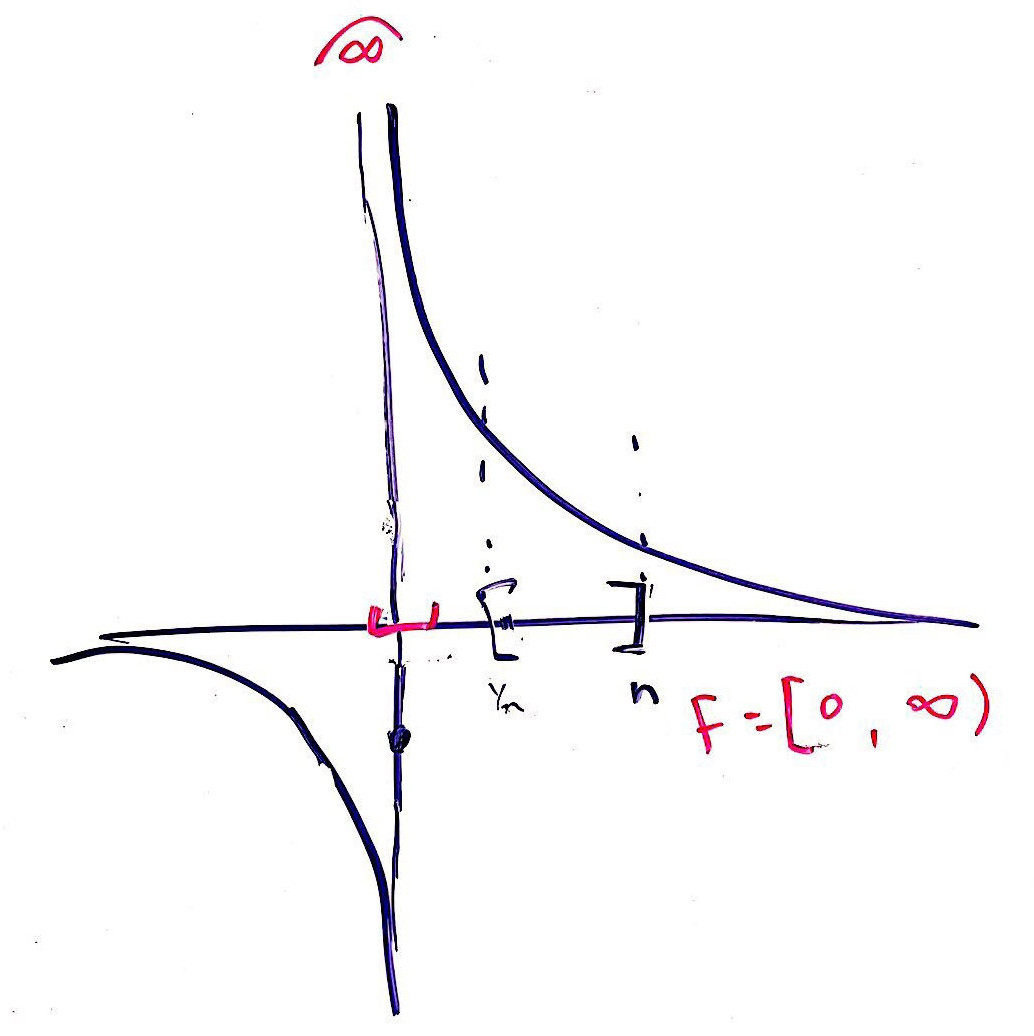
\includegraphics[width=0.2\textwidth]{final-1}
	\end{align*}
	\marginpar{
	\hspace{-1.3in}\vspace{-1in}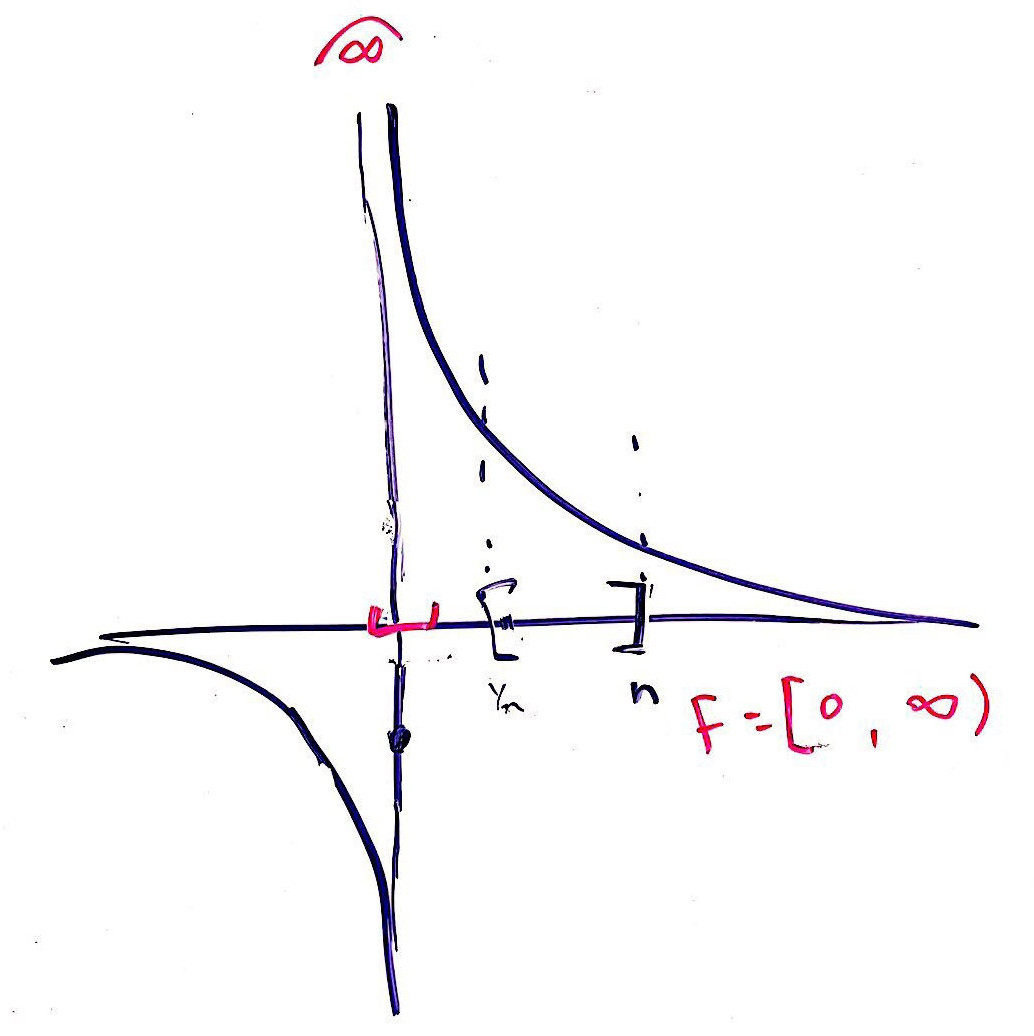
\includegraphics[width=2\marginparwidth]{final-1}
	%\captionof{figure}{Text of the caption}
	}
	
	and let $F=[0,\infty)$, $C_0=(-\infty,0]$, and for $n\in 1, 2, \dots$, $C_n=[\frac{1}{n},n]$. 
%	\jpg{width=0.2\textwidth}{final-1}
	Then $F,C_n$ are all closed, and $\bigcup_{n=0}^\infty C_n = \R$, with 
	$$\preimage{f|_{C_n}}{F}=\begin{cases}
	C_n, & n>0 \\
	\emptyset, & n=0
	\end{cases}
	$$
	which are all closed. But $\preimage{f}{F}=(0,\infty)$, which is not closed, so $f$ is not continuous. 
	\end{proof}

\pagebreak
\item \textit{Prove that if $f:M\to M$ is an isometry of a compact metric space, then $f$ is onto. (Recall that $f$ an isometry means $d\big(f(x), f(y)\big)=d(x,y)$ for all $x,y\in M$.)}
\begin{proof}
Suppose for contradiction there exists some $m\in M$ where $m\not\in f(M)$. Since $f$ is an isometry, then it is continuous\footnote{To see this, let $\delta=\varepsilon$ and use the $\delta$-$\varepsilon$ definition.}, so since $M$ is compact, then $f(M)$ is as well. Since $f(M)$ is a compact subset of a Hausdorff space, then it is closed. This means that $d(m,f(M))>0$\footnote{See the footnote in problem 4 for a proof of this fact.}, call this distance $\delta$. Now we make a sequence by iterating $f$, starting at $m$. Let 
\begin{align*}
m_0&=m, &m_n&=f(m_{n-1}) \quad \text{ for all } n\in\N.
\end{align*}
Since $m_1=f(m_0)\in f(M)$, then $d(m_0,m_1)\geq\delta$, and indeed $d(m_0,m_n)\geq\delta$ for all $n$ by the same reason. Since $f$ is an isometry, then $d(m_j,m_{n+j})=d(m_0,m_{n})\geq \delta$ for all $j,n\in\N$, so 
\begin{align*}
d(m_j,m_k)&\geq\delta \quad \text{whenever } j\neq k.
\end{align*}
However, since $M$ is compact then it is sequentially compact, so $\{m_n\}_{n=0}^\infty$ must have a subsequence $\{m_{n_i}\}_{i=0}^\infty$ which is convergent and thus Cauchy. So there exists some $I\in N$ such that for every $i,j>I$ with $i\neq j$, 
$$d(m_{n_i},m_{n_j})<\varepsilon \quad \text{ for any }\varepsilon>0,$$
a contradiction. 

\end{proof}

\vfill
\pagebreak
\item \textit{Give a careful definition of \emph{connected}. }
%\begin{definition*}
%Let $A\subseteq X$, where $X$ is a topological space. A \emph{separation} of $A$ is a pair of disjoint open sets which cover $A$ and neither set misses $A$. Symbolically, a separation is $U,V\in\script{T}_X$ s.t. \linebreak $U\cap A\neq\emptyset, V\cap A\neq\emptyset, U\cap V=\emptyset,$ and $ A \subseteq U\cup V.$
%\end{definition*}
\begin{definition*}
Let $X$ be a topological space. A \emph{separation} of $X$ is a pair of disjoint nonempty open sets which cover $X$. 
\end{definition*}
\begin{definition*}
Let $X$ be a topological space. $X$ is \emph{connected} if there does not exist a separation of $X$.%\footnote{I have given the definition of a \emph{connected subspace} here, since it is more general and I } 
\end{definition*}
%\textbf{Equivalent definition.} A topological space $X$ is \emph{connected} if there does not exist a continuous and onto function $f:A\to\{0,1\}$. (The codomain has the discrete topology.)

%That is, for any pair of sets $U,V\in X$, at least one of the following is true:
%	\begin{itemize}
%	\item $U\cap V\neq\emptyset$
%	\item one of $A, B$ is not open in $X$
%	\item $A\not\subset U\cup V$
%	\end{itemize}
	\begin{enumerate}
	\item \textit{Prove that the closed interval $[0,1]$ (with the usual topology) is connected. }
		\begin{proof}
		Suppose for contradiction that $A,B$ comprise a separation of $[0,1]$, and let 
		$$\alpha=\inf(A), \quad \beta=\inf(B).$$ 
		$A$ and $B$ are open sets in $[0,1]\subset \R$, so each is a countable union of disjoint intervals which are open in $[0,1]$. Thus one of $A,B$ contains $[0,x)$\footnote{If this is not obvious, note that $A,B$ are open in the subspace topology on $[0,1]$ which means there exist $U,V$ open in $\R$ such that $U\cap[0,1]=A$ and $V\cap[0,1]=B.$ So since $0\in U\cup V$, then $0\in(a,b)$ for some $(a,b)$ in either $U$ or $V$. Intersecting yields the desired $[0,b)$.} 
		for some $x\in(0,1)$, so \Wlog{} say that $A$ does, which means $\alpha=0$ and $\beta>0$. 
		
		\textbf{Claim. } $\beta\not\in A\cup B$, contradicting our assumption that $\{A,B\}$ is a separation of $[0,1]$. 
		\textbf{Proof of claim}
		Observe that $\beta\not\in B$, since if it were then some $B_\varepsilon(\beta)\subset B$, which means there exists some $x\in B$ such that $x<\beta$, contradicting that $\beta=\inf(B).$ 
		
		However $\beta\not\in A$ either, since if it were then some $B_\varepsilon(\beta)\subset A$. Since $\beta=\inf(B)$, any number greater than $\beta$ is not a lower bound for $B$, which means there exists some $x\in (\beta,\beta+\varepsilon)\subset B_\varepsilon(\beta)\subset A$ such that $x\in B$. This contradicts that $A$ and $B$ are disjoint. Therefore the claim is proved and the problem follows. 		
		\end{proof}
	\item \textit{Show that a connected metric space with at least two points is uncountable. }
	\begin{proof}
	Let $a_0$ and $a_\delta$ denote two points in the space $M$ where $\delta=d(a,b)$. The following claim produces an injective map from the interval $(0,\delta)$ to $M$, which means $|M|\geq |\R|$. 
	
	\textbf{Claim.} For every real number $x\in(0,\delta)$, there exists a point $a_x$ such that $a_x=a_y$ iff $x=y$. 
	
	\textbf{Proof of claim} Let $x\in(0,\delta)$ be given. Consider the sets
	\begin{align*}
	A_{<x}=\{a\in M : d(a_0,a) < x\}\\
	A_{>x}=\{a\in M : d(a_0,a) > x\}.
	\end{align*}
	They are open because $A_{<x}$ is an open ball and $B_{\delta-x}(a_\delta)\subset A_{>\delta}$. They are disjoint by definition, and they are nonempty because $a_0\in A_{<x}$ and $a_\delta\in A_{>x}$. Thus they 	are a pair of disjoint nonempty open sets, so they cannot cover $M$. This means 	
	\begin{align*}
	\left(A_{<x}\cup A_{>x}\right)^\complement&=\{a\in M : d(a_0,a) = x\} \\
	&\neq\emptyset,
	\end{align*}
	so there exists some $a_x\in M$ with $d(a_0,a_x)=x$. 
	
	Now for any $x,y\in(0,\delta)$ with $x\neq y$, we must have that $a_x\neq a_y$ since 
	\begin{align*}
	x=d(a_0,a_x), \quad
	y=d(a_0,a_y)
	\end{align*}
	and $d$ is a well-defined function. 
	\end{proof}
	\end{enumerate}
	
\vfill
\pagebreak
\item \textit{Let $\{C_n\}_{n\geq1}$ be a family of closed subsets of the compact metric space $X$ for which \linebreak $\bigcap_{n\geq1}C_n=\emptyset$. Prove that there is an $\varepsilon>0$ so that every ball in $X$ of radius $\varepsilon$ misses at least one $C_k$. }
\begin{proof} Since $\bigcap_{n\geq1}C_n=\emptyset$, then every $x\in X$ has some $C_n$ which does not contain it. So let 
$$\Gamma_x=\{n\in\N : x\not\in C_n\},$$
and for each $x\in X$ and $n\in \Gamma_x$, let 
$$\delta_{x,n}=\frac{1}{2}	d(x,C_n)=\frac{1}{2}\inf_{y\in C_n} d(x,y)$$
Note that each $\delta_{x,n}>0$, since $\{x\},$ and $C_n$ are disjoint closed sets and thus have positive distance\footnote{This is a common theorem about closed sets in metric spaces, but I don't believe we proved it in class. To see that it holds here, suppose that $x\not\in C_n$ and $d(x,C_n)=0$. Then every ball $B_\varepsilon(x)$ contains some point in $C_n$ because $\varepsilon$ is not a lower bound for $\{d(x,y):y\in C_n\}$, so $x\in \closure{C_n}=C_n$, contradiction.}. 
This means that the collection of open balls 
$$\{B_{\delta_{x,n}}(x) : {x\in X, n\in\Gamma_x} \}$$
is an open cover of $X$, and thus has a finite subcover, call it $\{B_{\delta_i}(x_i)\}_{i=1}^N.$ If we let 
$$\delta=\min(\delta_i),$$
Then any ball of radius $\delta$ misses at least one $C_n$. To see this, let $x\in X$. Since $\{B_{\delta_i}(x_i)\}_{i=1}^N$ is an open cover of $X$, there exists some $B_{\delta_j}(x_j)$ containing x, so
$$d(x_j,x)<\delta_j.$$
Since $\delta_j=\delta_{x_j,n_j}$ for some $n_j\in\Gamma_{x_j}$, then 
$$d(x_j,C_{n_j})=2\delta_j,$$
so by the Triangle Inequality, 
\begin{align*}
d(x,C_n) &\geq d(x_j,C_{n_j})-d(x_j,x) \\
&\geq 2\delta_j - \delta_j \\
&=\delta_j \\
&\geq\delta
\end{align*}
and $B_\delta(x)$ misses $C_{n_j}$. 
\end{proof}

\vfill
\pagebreak
\item \textit{Define what it means for a metric space to be \emph{complete}.}
\begin{definition*}
Let $(M,d)$ be a metric space. We say $M$ is \emph{complete} if every Cauchy sequence in $M$ converges to a point in $M$. 
\end{definition*}
\textit{State carefully and prove the contraction mapping theorem for metric spaces. }
\begin{theorem*}\textbf{(Contraction Mapping Theorem)}
In a complete metric space, every contraction has a fixed point. That is, let $(M,d)$ be a complete metric space and let $f:M\to M$ be a function with the property that  
$\text{for all }x,y\in M\text{, there exists }\lambda\in(0,1)\text{ such that }d\big(f(x),f(y)\big)\leq\lambda d(x,y).$
%
Then there exists a unique $x\in M$ with $f(x)=x$. 
\end{theorem*}
\begin{proof}
Let $x_0$ be any element in $M$. As we did in problem 2, we iterate: let $x_n=f(x_{n-1})$ for all $n\in\N$, and call $\delta=d(x_0,x_1)$. Then $d(x_n,x_{n+1})\leq \lambda^n\delta$, which means that for all $n<m\in\N$,
\begin{align*}
d(x_n,x_m)&\leq\sum_{i=n}^{m-1}d(x_i,x_{i+1})\\
&\leq \sum_{i=n}^{m-1} \lambda^i\delta\\
&\leq \sum_{i=n}^{\infty} \lambda^i\delta,\\
%&=\frac{\delta}{1-\lambda}
\end{align*} 
which is a tail of a convergent geometric series, so for any $\varepsilon>0$, there exists some $N\in\N$ such that
\begin{align*}
\epsilon &> \sum_{i=N}^{\infty} \lambda^i\delta \\
&\geq d(x_n,x_m) \quad \text{if }n,m>N.
\end{align*}
Thus, $\{x_n\}_{n=0}^\infty$ is a Cauchy sequence in $M$. Since $M$ is complete, then $\{x_n\}_{n=0}^\infty$ converges to a point in $M$, and we can call the limit $x$. To see that $f(x)=x$, first note that $f$ is continuous at every point $a\in M$, since for every $\varepsilon>0$ if $d(a,b)<\frac{\varepsilon}{\lambda}=\delta$, then $d\big(f(a),f(b)\big)<\varepsilon$. Now suppose that $f(x)=y\neq x$, and let $\epsilon=\frac{d(x,y)}{\Omega}$ for some large number $\Omega>\frac{1}{\lambda}+1$.  Then $\delta=\frac{d(x,y)}{\Omega\lambda}$ and whenever ${d(x,a)<\delta}$, then $d(y,f(a))<\frac{d(x,y)}{\Omega}$. But we can find some $n$ such that $d(x,x_n)<\delta$, which means that both 
\begin{align*}
d(y,x_{n+1})&<\frac{d(x,y)}{\Omega} \quad \text{by continuity, and} \\
d(x,x_{n+1})&<\frac{d(x,y)}{\Omega\lambda} \quad \text{since }x_n\to x,
\end{align*}
Which contradicts the Triangle Inequality, since 
$d(y,x_{n+1}) + d(x,x_{n+1}) < \tfrac{d(x,y)}{\Omega} + \tfrac{d(x,y)}{\Omega\lambda} < d(x,y).$ Finally, note that this fixed point is unique since if $x\neq y$ and $x,y$ are fixed points, then ${d(f(x),f(y))=d(x,y)\not\leq\lambda d(x,y)}$.
\end{proof}


\textit{Show that if $f(x)$ is a real differentiable function with $|f'(x)|<M$ for all real $x$, then for any real numbers $a_{ij}$ and $b_{j}$, there is one and only one point $(x_1, \dots, x_n)$ satisfying
$$x_i=\sum_{j=1}^na_{ij}f(x_j)+b_j \quad \text{where } 1\leq i\leq n,$$
provided that 
$$\sum_{i,j}a_{ij}^2<1/M^2.$$}
\begin{proof}
Let $f:\R\to\R$ be a function with the above properties, let $\mathbf{A}\in M_n(\R)$ with entries given by the numbers $a_{ij}$ above, and let $\vec{b}\in\R^n$ be have $\sum_{j=1}^n b_j$ in every coordinate. Let $\varphi:\R^n\to\R^n$ be $\varphi(\vec{x})=(f(x_1), \dots, f(x_n))$ Finally let $\Phi:\R^n\to\R^n$ be
$$\Phi(\vec{x})=\mathbf{A}\varphi(\vec{x})+\vec{b}.$$
Since $\R^n$ equipped with the Euclidean metric is complete, we will show that $\Phi$ is a contraction, and by applying the Contraction Mapping Theorem, we will be done. 

We can write $\Phi(\vec{x})$ as 
\begin{align*}
\Phi(\vec{x})&=\mathbf{A}\varphi(\vec{x})+\vec{b}\\
&=
	\left[
	\begin{array}{ccccc}
	a_{11} & \cdots & a_{1j} & \cdots & a_{1n} \\
	\vdots & \ddots &        &        & \vdots \\
	a_{i1} &        & a_{ij} &        & a_{in} \\
	\vdots &        &        & \ddots & \vdots \\
	a_{n1} & \cdots & a_{nj} & \cdots & a_{nn} 
	\end{array}
	\right]
%
	\left[
	\begin{array}{c}
	f(x_1) \\
	\vdots \\
	f(x_i) \\
	\vdots \\
	f(x_n) 
	\end{array}
	\right]
+
	\left[
	\begin{array}{c}
	\sum_{j=1}^n b_j \\
	\vdots \\
	\sum_{j=1}^n b_j \\
	\vdots \\
	\sum_{j=1}^n b_j 
	\end{array}
	\right]
\\
&=
	\left[
	\begin{array}{c}
	\sum_{j=1}^n \big(a_{1j}f(x_j)+b_j\big) \\
	\vdots \\
	\sum_{j=1}^n \big(a_{ij}f(x_j)+b_j\big) \\
	\vdots \\
	\sum_{j=1}^n \big(a_{nj}f(x_j)+b_j\big) 
	\end{array}
	\right]
\end{align*}
so for any $\vec{x},\vec{y}\in\R^n$, the $i$-th coordinate of $\Phi(\vec{x})-\Phi(\vec{y})$ is given by 
\begin{align*}
\pi_i\big(\Phi(\vec{x})-\Phi(\vec{y})\big)
&= 
	\sum_{j=1}^n \big(a_{ij}f(x_j)+b_j\big) 
	-
	\sum_{j=1}^n \big(a_{ij}f(y_j)+b_j\big) 
%\\&=
%	\sum_{j=1}^n \big(a_{ij}f(x_j)\big)
%	-
%	\sum_{j=1}^n \big(a_{ij}f(y_j)\big)
%\\&=
%	\sum_{j=1}^n \big(a_{ij}f(x_j) -	a_{ij}f(y_j)\big)
\\&=  \sum_{j=1}^n a_{ij}\big(f(x_j) -	f(y_j)\big)
\end{align*}
and now we check that the squared distance $\norm{\Phi(x)-\Phi(y)}^2$ is bounded by $\norm{\vec{x}-\vec{y}}^2$, 
\begin{align*}
\sum_{i=1}^n \big[\pi_i\big(\Phi(\vec{x})-\Phi(\vec{y})\big)\big]^2
&= \sum_{i=1}^n \left(\sum_{j=1}^n a_{ij}\big(f(x_j) -	f(y_j)\big)\right)^2 
	& \text{and by Cauchy-Schwarz,}\\
&\leq
	\sum_{i=1}^n \left( 
	\left(\sum_{j=1}^n a_{ij}^2\right)
	\left(\sum_{j=1}^n\big(f(x_j) -	f(y_j)\big)^2\right) 
	\right)
	& \begin{array}{r}
	\text{and since right hand } \\
	\text{factor is constant w.r.t. }i,
	\end{array}	 \\
&\leq
	\left(\sum_{i,j} a_{ij}^2\right)
	\left(\sum_{j=1}^n\big(f(x_j) -	f(y_j)\big)^2\right) 
	& \text{and since } \sum_{i,j} a_{ij}^2<\frac{1}{M^2}, \\
&= \frac{\lambda}{M^2}
	\left(\sum_{j=1}^n (x_j -	y_j)^2 \left(\frac{f(x_j) -	f(y_j)}{x_j -	y_j}\right)^2\right)
	& \text{and since } |f'(x)|<M,\footnotemark\\
&< \frac{\lambda}{M^2}
	\left(\sum_{j=1}^n (x_j -	y_j)^2 M^2\right) \\
&= \lambda\sum_{j=1}^n (x_j -	y_j)^2 \\
&=\lambda\norm{\vec{x}-\vec{y}}^2,
\end{align*}
where $\lambda=M^2\sum_{j=1}^n a_{ij}^2<1$. Thus  \footnotetext{The difference quotient can't exceed the bound on the derivative since the Mean Value Theorem guarantees a point where the derivative is equal to the difference quotient.}
$$\norm{\Phi(x)-\Phi(y)}^2<\lambda \norm{\vec{x}-\vec{y}}^2,$$
so $\Phi$ is a contraction, and thus has a unique fixed point.\footnote{I didn't expect to have to dig out my Linear Algebra knowledge from the old mental closet, and it was fun. I thoroughly enjoyed this problem.}
\end{proof}
\vfill
\pagebreak
\end{enumerate}
\end{document}



